% !TEX root = ../main.tex

\chapter{Makefile and CMake}

\section{Large Project Structure}

When working on a large project, it is essential to organize your repository in a way that makes it easy to manage and understand. A typical structure might look like this:

\begin{itemize}
    \item \textbf{src/}: Contains all the source code files.
    \item \textbf{include/}: Contains all the header files.
    \item \textbf{lib/}: Contains external libraries.
    \item \textbf{build/}: Directory where the build system generates output files.
    \item \textbf{tests/}: Contains test code and test data.
    \item \textbf{docs/}: Contains documentation files.
    \item \textbf{CMakeLists.txt}: The main CMake configuration file.
    \item \textbf{README.md}: A file that provides an overview of the project.
\end{itemize}

This structure helps in maintaining a clean and organized codebase, making it easier for multiple developers to collaborate and for new developers to get up to speed quickly.

\begin{figure}[H]
    \centering 
    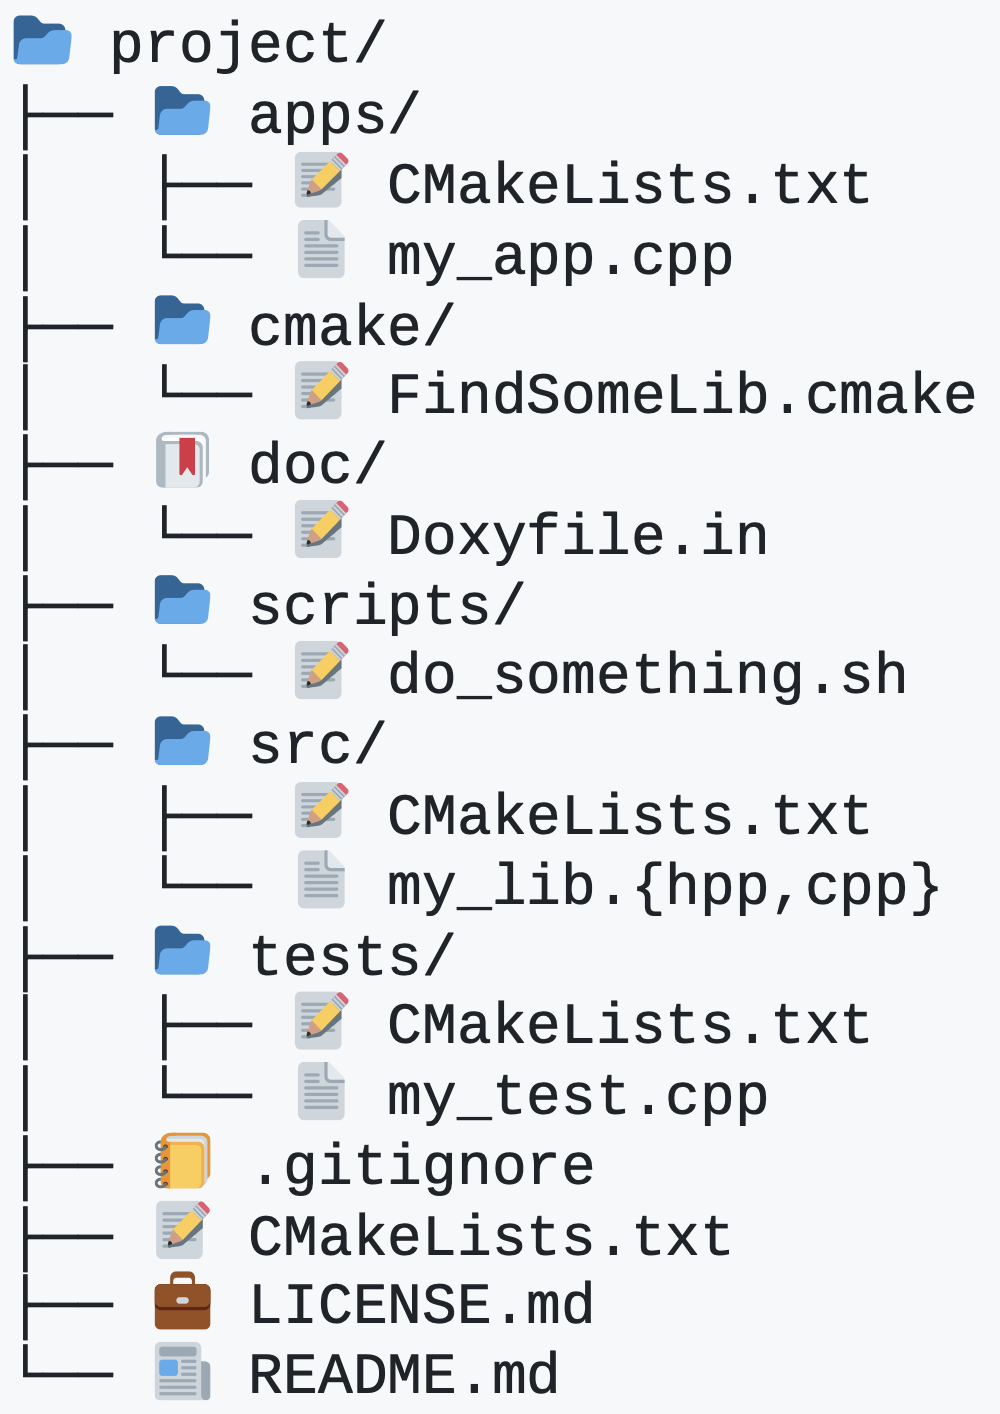
\includegraphics[width=0.4\textwidth]{assets/large_project.png}
    \caption{large Project Structure}
\end{figure}

\newpage
\section{Makefile}


A \texttt{Makefile} can automate compilation and linking processes for your project. make efficiently determines the need to regenerate a target by checking its existence and the up-
to-dateness of prerequisite files. This feature enables it to avoid unnecessary target regeneration.
Make simplifies the installation of numerous libraries through a concise set of commands. A typical
sequence for installing an open-source library involves using the following commands:

\begin{codeblock}[language=bash]
    make  ##builds the library
    make install   ##copies the library's headers, the libraries and the binaries to a user-specified folder
\end{codeblock}

\begin{itemize}
    \item \textbf{Target:} represents the desired output or action. It can be an executable, an
object file, or a specific action like "clean."
    \item \textbf{Prerequisites:} are files or conditions that a target depends on. If any of the prerequisites have
been modified more recently than the target, or if the target does not exist, the associated
recipe is executed.
    \item \textbf{Recipes:} is a set of shell commands that are executed to build or update the target.
\end{itemize}

Considering a very simple case where we only have three files (math.hpp, math.cpp and main.cpp), we can write:

\begin{codeblock}[language=bash]
main.o: main.cpp math.hpp   ## for compilation of main.cpp
    g++ std=c++17 -Wall main.cpp -c
math.o: math.cpp math.hpp   ## for compilation of math.cpp
    g++ -std=c++17 -Wall math.cpp -c
main: main.o math.o   ## for linking
    g++ main.o math.o -o main
clean:   ## for cleaning object files
    rm -rf main *.o
\end{codeblock}

Take for example the first line of code, \texttt{main.o: main.cpp math.hpp}. This line tells make that the target \texttt{main.o} depends on the files \texttt{main.cpp} and \texttt{math.hpp}. If either of these files has been modified more recently than \texttt{main.o}, make will execute the recipe associated with this target. The recipe is the set of shell commands that follow the target definition.

A Makefile only redo the operations that contains files that have changed, and one can also call a single recipe instead of the entire file.


Use then variables for clarity and maintainability (used with \$(...))

\begin{codeblock}[language=bash]
CXX=g++
CPPFLAGS=-I.   ## for the preprocessor of either C++ or C
CXXFLAGS=-std=c++17 -Wall -Wpedantic -Werror   ## specific for c++ compiler

main.o: main.cpp math.hpp   ## for compilation
    $(CXX) $(CPPFLAGS) $(CXXFLAGS) main.cpp -c
math.o: math.cpp math.hpp   ## for compilation
    $(CXX) (CPPFLAGS) $(CXXFLAGS) math.cpp -c
main: main.o math.o   ## for linking
    $(CXX) $(CXXFLAGS) main.o math.o -o main
clean:   ## for cleaning object files
    rm -rf main *.o

\end{codeblock}
since the first two commands are the same we can summarize them:
\begin{codeblock}[language=bash]
CXX=g++
CPPFLAGS=-I.   ## for the preprocessor of either C++ or C
CXXFLAGS=-std=c++17 -Wall -Wpedantic -Werror   ## specific for c++ compiler

all=main  ## convention used to specify the final target of the project

%.o: %.cpp math.hpp
    $(CXX) $(CPPFLAGS) $(CXXFLAGS) $< -c
main: $(OBJS)   ## for linking
    $(CXX) $(CXXFLAGS) $^$ -o $@
    ## $@ stands for the target file
    ## $^ expands to the list of all prerequisites (dependencies) of the current target
clean:   ## for cleaning object files
    rm -rf *.o
\end{codeblock} 

Now we can introduce the variables \texttt{DEPS}, \texttt{SRCS} and \texttt{OBJS} to make the Makefile more general:
\begin{codeblock}[language=bash]
CXX=g++
CPPFLAGS=-I.   ## for the preprocessor of either C++ or C
CXXFLAGS=-std=c++17 -Wall -Wpedantic -Werror   ## specific for c++ compiler

DEPS=math.hpp
SRCS=$(wildcard *.cpp)  ##List of all .cpp files
OBJS=$(SRCS:.cpp=.o)  ##Same, but replace .cpp with .o

all=main  ## convention used to specify the final target of the project

%.o: %.cpp $(DEPS)
    $(CXX) $(CPPFLAGS) $(CXXFLAGS) $< -c
main: main.o math.o   ## for linking
    $(CXX) $(CXXFLAGS) $^$ -o $@
    ## $@ stands for the target file
    ## $^ expands to the list of all prerequisites (dependencies) of the current target
clean:   ## for cleaning object files
    rm -rf *.o
\end{codeblock}

To use this \texttt{Makefile}, simply type:

\begin{codeblock}[language=bash]
make
\end{codeblock}

To clean up:

\begin{codeblock}[language=bash]
make clean
\end{codeblock}

Example with dynamic library:
\begin{exampleblock}[Library Makefile]
\begin{codeblock}[language=bash]
    ### Library Makefile
    CXX=g++
    CPPFLAGS=-I.
    CXXFLAGS=-std=c++17 -Wall -Wpedantic -Werror
    
    SRC=$(wildcard *.cpp)
    OBJ=$(SRC:.cpp=.o)
    OBJ_fPIC=$(SRC:.cpp=.fpic.o)
    DEPS=$(wildcard *.h)
    
    LIB_NAME_SHARED=libparser.so
    
    all: shared 
    shared: $(LIB_NAME_SHARED)
    
    $(LIB_NAME_SHARED): $(OBJ_fPIC)
    	g++ $(CXXFLAGS) -shared $^ -o $@
    
    %.fpic.o: %.cpp $(DEPS)
    	$(CXX) -c -fPIC $(CPPFLAGS) $(CXXFLAGS) $^ -o $@
    
    %.o: %.cpp $(DEPS)
    	$(CXX) -c $(CPPFLAGS) $(CXXFLAGS) $^ -o $@
    
    clean:
    	rm -f *.o $(LIB_NAME_SHARED)
\end{codeblock}
\end{exampleblock}
\begin{exampleblock}[Project Makefile]
\begin{codeblock}[language=bash]
    ### Project Makefile
    CXX=g++
    CPPFLAGS=-Iparser/
    CXXFLAGS=-std=c++17 -Wall -Wpedantic -Werror
    
    LDFLAGS=-Wl,-rpath,parser/ -Lparser/ # For dynamic linking.
    LDLIBS=-lparser # Link the shared library libparser.so
    
    SRC=ex1.cpp 
    OBJ=$(SRC:.cpp=.o)
    
    all: main
    
    main: $(OBJ)
    	$(CXX) $(CXXFLAGS) $^ $(LDFLAGS) $(LDLIBS) -o $@
    
    %.o: %.cpp
    	$(CXX) -c $(CPPFLAGS) $(CXXFLAGS) $< -o $@
    
    clean:
    	rm -f *.o main
\end{codeblock}
\end{exampleblock}
Then run in the terminal:
\begin{codeblock}[language=bash]
    ### In the library directory:
    make

    ### In the project directory:
    make

    ### Now you can run the executable:
    ./main
\end{codeblock}


\section{CMake}

\subsection*{Introduction}

CMake stands for "Cross-Platform Make." It is a \textbf{build-system generator}, meaning it creates the files (e.g., \texttt{Makefile}, Visual Studio project files) needed by your build system to compile and link your project.
CMake abstracts away platform-specific build configurations, making it easier to maintain code that needs to run on multiple platforms.

It works the following way:
\begin{enumerate}
    \item You write a \texttt{CMakeLists.txt} file that describes your project's configuration and structure.
    \item You run CMake on the \texttt{CMakeLists.txt} file to generate the build system files (e.g. \texttt{Makefile} on Linux or .snl for Visual Studio).
    \item You use the generated build system to compile and link your project.
\end{enumerate}

\subsection*{CMakeLists.txt}

Contains the configuration and structure of your project. It is a script that CMake uses to generate the build system files.
It has the following structure:

\begin{codeblock}[language=bash]
cmake_minimum_required(VERSION 3.12) 
project(MyProject VERSION 1.0
    DESCRIPTION "My Project"
    LANGUAGES CXX)
\end{codeblock}

\begin{warningblock}
    Use a CMake version more recent than your compiler (e.g., CMake 3.12 for C++17).

    Also, command names are \textbf{case insensitive}.
\end{warningblock}

\subsubsection{Minimum Version}

Here is the first line of every \texttt{CMakeLists.txt}, which is the required name of the file CMake looks for:
\begin{codeblock}[language=bash]
cmake_minimum_required(VERSION 3.10)
\end{codeblock}
The version on CMake dictates the policies. Starting in CMake 3.12, this supports
a range like \texttt{3.12...3.15}. This is useful when you want to use new features but still support older versions.
\begin{codeblock}[language=bash]
cmake_minimum_required(VERSION 3.12...3.15)
\end{codeblock}

\subsubsection{Setting a project}
Every top-level CMake file will have this line:
\begin{codeblock}[language=bash]
project(MyProject VERSION 1.0
    DESCRIPTION "My Project"
    LANGUAGES CXX)
\end{codeblock}

Strings are quoted, whitespace does not matte and the name of the prokect is the first argument.
All the keywords are optional. The \texttt{version} sets a bunch of variables, like \texttt{MyProject\_VERSION} 
and \texttt{PROJECT\_VERSION}. The \texttt{LANGUAGES} keyword sets the languages that the project will use. This is useful for IDEs that support multiple languages.

\subsubsection{Making an executable}

\begin{codeblock}[language=bash]
add_executable(my_project_main my_project_main.cpp)
\end{codeblock}

\texttt{my\_project} is both the name of the executable file generate and the name of the CMake target created.
The source file comes next and you can add more than one source file. CMake will only compile source file extensions. 
The headers will be ignored for most purposes; they are there only to be showed up in IDEs.

\subsubsection{Making a library}

\begin{codeblock}[language=bash]
add_library(my_library STATIC my_library.cpp)
\end{codeblock}

\texttt{STATIC} is the type of library. It can be \texttt{SHARED} or \texttt{MODULE}. The source files are the same as for executables.
Often you'll need to make a fictional target, i.e., one where nothing needs to be compiled, for example for header-only libraries. This is called an \texttt{INTERFACE library},
and the only difference is that it cannot be followed by filenames.

\subsubsection{Targets}

Now we've specified a target, we can set properties on it.
CMake is all about targets and properties. An executable is a target, a library is a target. Your
application is built as a collection of targets depending on each other.


\begin{codeblock}[language=bash]
target_include_directories(my_library PUBLIC include)
\end{codeblock}

This sets the include directories for the target. The \texttt{PUBLIC} keyword means that the include directories will be propagated to any target that links to \texttt{my\_library}.
We can then chain targets:

\begin{codeblock}[language=bash]
add_library(my_library STATIC my_library.cpp)
target_link_libraries(my_project PUBLIC my_library)
\end{codeblock}

This will link \texttt{my\_project} to \texttt{my\_library}. The \texttt{PUBLIC} keyword means that the link will be propagated to any target that links to \texttt{my\_project}.

Targets can have include directories, linked libraries (or linked targets), compile options, compile definitions, 
compile features and more.

\subsubsection*{Basic Example}
\begin{exampleblock}
\begin{codeblock}[language=bash]
cmake_minimum_required(VERSION 3.10)
project(Libraries_Tests)

# First create the static or shared library, in this case the project contains the library
add_library(chrislib_static STATIC src/chrislib.cpp)
add_library(chrislib_shared SHARED src/chrislib.cpp)

# Then create the executable of the main file
add_executable(main_static src/main.cpp)
add_executable(main_shared src/main.cpp)

# Set the properties of the libraries, in this case the include directories
target_include_directories(chrislib_static PUBLIC include)
target_include_directories(chrislib_shared PUBLIC include)

# Link the libraries to the executables
target_link_libraries(main_static chrislib_static)  
target_link_libraries(main_shared chrislib_shared)

# (Optional) Create custom commands to run the executables 
add_custom_target(run_static
    COMMAND main_static
    DEPENDS main_static
    WORKING_DIRECTORY ${CMAKE_PROJECT_DIR}
)

add_custom_target(run_shared
    COMMAND main_shared
    DEPENDS main_shared
    WORKING_DIRECTORY ${CMAKE_PROJECT_DIR}
)

# Clean
add_custom_target(clean_all
    COMMAND rm -f ../build/* ../lib/*
)
\end{codeblock}
\end{exampleblock}

\subsubsection*{Control Flow}

\begin{codeblock}[language=bash]
if (MY_VAR)
    message(STATUS "MY_VAR is set")
else()
    message(STATUS "MY_VAR is not set")
endif()
\end{codeblock}

Many operators can be used in the if statement, like \texttt{AND}, \texttt{OR}, \texttt{NOT}, \texttt{EQUAL}, \texttt{LESS}, \texttt{GREATER}, \texttt{MATCHES} and \texttt{IN\_LIST}.
You can also use \texttt{foreach}, \texttt{while} and \texttt{function}. 

With \textbf{branch selection} (using \texttt{if} and \texttt{\#ifdef} statements), you can switch among different implementations or versions of any third-party library. 
This is useful when you want to use different implementations of a library depending on the platform or the compiler. 
As an example, 
\begin{codeblock}[language=bash]
#ifdef USE_BOOST
    #include <boost/algorithm/string.hpp>
#else
    #include <algorithm>
#endif
\end{codeblock}

But how to choose the correct branch? You can use the \texttt{option} command:

\begin{codeblock}[language=bash]
option(USE_BOOST "Use Boost library" ON)
\end{codeblock}

This will create a cache variable that can be set from the command line. If you want to set it from the command line, you can use the \texttt{-D} flag:

\begin{codeblock}[language=bash]
cmake /path/to/src/ -DUSE_BOOST=OFF
\end{codeblock}


\subsubsection{Variables}

\texttt{Local variables} are used to store values that are used only in the current scope:

\begin{codeblock}[language=bash]
set(MY_VAR "some_file") 
\end{codeblock}

The names of the variables are case-sensitive and the values are strings. You access a variable by using \texttt{\$\{\}}.
CMake has the concept of scope; you cna access the value of the variable after you set it as long as you are in the same scope. If you leave a function or a file in a sub directory, the variable will 
no longer be defined. You can set a variable in the scope immediately above your current one with \texttt{PARENT\_SCOPE} at the end. 

One can also set a list of values:

\begin{codeblock}[language=bash]
set(MY_LIST "value1" "value2" "value3")
\end{codeblock}

which internally becomes a string with semicolons. You can access the values with \texttt{\$\{MY\_LIST\}}.

If you want to set a variable from the command line, CMake offers a variable cache.
\texttt{Cache variables} are used to interact with the command line:

\begin{codeblock}[language=bash]
set(MY_CACHE_VAR "VALUE" CACHE STRING "Description")

option(MY_OPTION "Set from command line" ON)
\end{codeblock}

Then:
\begin{codeblock}[language=bash]
cmake /path/to/src/ \
-DMY_CACHE_VAR="some_value" \
-DMY_OPTION=OFF
\end{codeblock}

\texttt{Environment variables} are used to interact with the environment:

\begin{codeblock}[language=bash]
# Read
message(STATUS $ENV{MY_ENV_VAR})

# Write
set(ENV{MY_ENV_VAR} "some_value")
    
\end{codeblock}

But it is not recommended to use environment variables in CMake.

\subsubsection{Properties}

The other way to set properties is to use the \texttt{set\_property} command:

\begin{codeblock}[language=bash]
set_property(TARGET my_library PROPERTY CXX_STANDARD 17)
\end{codeblock}

This is like a variable, but it is attached to a target. The \texttt{PROPERTY} keyword is optional. The \texttt{CXX\_STANDARD} is a property that sets the C++ standard for the target.

\begin{observationblock}
    We personally suggest to go deeper in the CMake arguments and properties, since listing every possible 
    command here would be too long. The above examples are the most common ones but contain all the basic
    information to start using CMake.
\end{observationblock}

Just for the sake of completeness, below is a more complete example of a \texttt{CMakeLists.txt} file which uses GTest and compiles multiple source files:
It compiles the main engine and the tests, linking them with Google Test and creating a custom target to run the executable.

\begin{exampleblock}
\begin{codeblock}[language=bash]
cmake_minimum_required(VERSION 3.10)
# Project name
project(ChessEngine)
# Set C++ standard
set(CMAKE_CXX_STANDARD 17)
set(CMAKE_CXX_STANDARD_REQUIRED True)

# Include directories
include_directories(${PROJECT_SOURCE_DIR}/include)

# Source files
set(SOURCES
    src/*.cpp
)

# Add executable for main engine
add_executable(ChessEngine src/main.cpp ${SOURCES})

# Google Test setup
enable_testing()
find_package(GTest REQUIRED)

# Add test sources
set(TEST_SOURCES
    test/test.cpp
)

# Create test executable
add_executable(ChessEngineTests ${TEST_SOURCES} ${SOURCES})

# Link test executable with Google Test and required libraries
target_link_libraries(ChessEngineTests GTest::GTest GTest::Main pthread)

# Add test to CTest framework
add_test(NAME ChessEngineTests COMMAND ChessEngineTests)

# Running executable
add_custom_target(play
    COMMAND ChessEngine
    DEPENDS ChessEngine
    WORKING_DIRECTORY ${CMAKE_PROJECT_DIR}
)

# (Optional)Cleaning
add_custom_target(clean-all
    COMMAND ${CMAKE_BUILD_TOOL} clean
    COMMAND rm -rf CMakeFiles CMakeCache.txt cmake_install.cmake Makefile
    COMMAND rm ../build/*
    WORKING_DIRECTORY ${CMAKE_PROJECT_DIR}
)
\end{codeblock}
\end{exampleblock}